\documentclass[iop]{emulateapj}

\usepackage{amsmath,amssymb}
\usepackage{color}
\usepackage{natbib}
\usepackage{graphicx}
\usepackage{hyperref}
\usepackage{ulem}
\usepackage{adjustbox}
\usepackage[draft]{todonotes}

\newcommand\toplotrm[1]{\todo[color=green, inline, size=\small]{Plot: #1}}
\newcommand\towriterm[1]{\todo[color=yellow, inline, size=\small]{Write: #1}}
\newcommand\todorm[1]{\todo[color=cyan, inline, size=\small]{To do: #1}}

\newcommand\toplotemh[1]{\todo[color=pink, inline, size=\small]{Plot: #1}}
\newcommand\towriteemh[1]{\todo[color=orange, inline, size=\small]{Write: #1}}
\newcommand\todoemh[1]{\todo[color=red, inline, size=\small]{To do: #1}}

\newcommand\towrite[1]{\todo[color=gray, inline, size=\small]{Write: #1}}


\citestyle{aa}

\shorttitle{Meta-Calibration} \shortauthors{Huff and Mandelbaum}

\begin{document}
\title{Meta-Calibration: Direct Self-Calibration of Biases in Shear Measurement}
\author{Eric M. Huff\altaffilmark{1}}
\author{Rachel Mandelbaum\altaffilmark{2}}

\altaffiltext{1}{Center for Cosmology and Astroparticle Physics, 
Department of Physics, The Ohio State University, OH 43210, USA}
\altaffiltext{2}{McWilliams Center for Cosmology, Department of Physics, Carnegie Mellon University,
  Pittsburgh, PA 15213, USA}

\keywords{cosmology: observations --- gravitational lensing: weak ---
  methods: observational}

\begin{abstract}
  One of the primary limiting sources of systematic error in forthcoming
  weak lensing measurements is systematic uncertainty in the
  quantitative relationship between the distortions due to
  gravitational lensing and the measurable properties of galaxy
  images. We present a statistically principled, general solution to
  this problem. Our technique infers calibration parameters for an
  arbitrary shape measuremtoent technique by modifying the real images
  to simulate the effects a known shear. We test our results on
  simulated timages from the Great3 shear calibration challenge, and
  show that the method eliminates calibration biases for a variety of
  shape measurement techniques at the level of precision measurable
  with the available Great3 simulations.
\end{abstract}



\section{Introduction}


Accurate measurement of weak gravitational lensing offers the most
direct probe of the dark sector of the universe
\citep[e.g.,][]{2001PhR...340..291B,2003ARA&A..41..645R,schneider06,2008ARNPS..58...99H,2010RPPh...73h6901M,2013PhR...530...87W}.
Weak lensing measurements are thus a core part of the international
cosmology program, and a key science driver for many wide-field
astronomical astronomical surveys (KiDS, DES, SuMIRE,
LSST\footnote{\url{http://www.lsst.org/lsst/}},
Euclid\footnote{\url{http://sci.esa.int/euclid/}\url{http://www.euclid-ec.org}}
\citep{2011arXiv1110.3193L},
WFIRST-AFTA\footnote{\url{http://wfirst.gsfc.nasa.gov}}
\citep{2009arXiv0912.0201L,2011arXiv1110.3193L,2015arXiv150303757S}).

Despite this investment, it is not yet clear that the statistical
power of these measurements will ultimately be matched by their
accuracy. There are several sources of systematic uncertainty that may
turn out to be larger than the statistical errors of these
experiments. One of the largest such systematic error sources is the
{\it shear calibration bias}, the quantitative realationship between
the gravitational lensing signal and its chief observables.

The major physical effect studied by weak lensing surveys is the
 gravitational shear. The major observable effect of a weak shear
$\boldsymbol{\gamma}$ is a perturbation to the observed ellipticities
$\boldsymbol{e}$ of distant galaxies. The intrinsic properties of
galaxies know no preferred direction, so their average ellipticity
$\boldsymbol{e}$ should vanish over a wide enough field. Weak lensing
measurements exploit this intrinsic symmetry, and search for
statistical anisitropies resulting from lensing distortions due to
foreground matter.

In the domain of weakest lensing, which is the major focus for
dark energy measurements, shears linearly modify the observed
ellipticities, and the calibration problem is quantitatively reduced
to constraining the coefficients of the linear relation
\begin{align}
\boldsymbol{e} = (1+m)\:\boldsymbol{\gamma} + c.
\end{align}
Generally $c$ is a result of measurement biases (such as an incomplete
correction for the point-spread function) that introduce a preferred
direction in the image plane. It can in principle be known or removed
with sufficient knowledge of the experiment. $m$ depends in part on
the ensemble of (unobserved) galaxy properties, so it is impossible in
principle to know exactly {\it a priori}.

In practice, nonlinearities introduced by the algorithms used for
measurement of $\boldsymbol{e}$ can introduce both multiplicative and
additive biases in a manner that interacts with the unknown true
ensemble properties of galaxies. and are very difficult to predict
from first principles. For this reason, the weak lensing community has
organized a series of blind measurement challenges, where participants
attempted to extract an unkown lensing signal from simulated images.
The earliest of these were the first two Shear TEsting Programmes
\citep[STEP1,STEP2]{2006MNRAS.368.1323H,2007MNRAS.376...13M}. The
results made two things clear: that lensing measurement algorithms
needed to improve, and that shear measurement was complex enough that
successive simulation challenges should focus on a subset of the
issues.

The next round of simulation challenges, GREAT08, GREAT10, and GREAT3,
\citep{2009AnApS...3....6B,2013ApJS..205...12K,2015MNRAS.450.2963M}
embraced a narrower focus and saw significant performance
improvements. In particular, the best-performing algorithms from the
most recent challenge, GREAT3, were able to reduce $m$ and $c$ to
levels that are good enough for even the most ambitious planned
lensing measurements.

While this was certainly good news, the narrowed focus of the GREAT
challenges necessarily left some of the most important sources of
lensing calibration bias untouched. Remaining issues of significant
concern include biases resulting from:
\begin{itemize}
\item object detection and selection
\item deblending
\item wavelength-dependent effects
\item instrumental defects and nonlinearities
\item star-galaxy separation
\item non-white pixel noise
\item cosmic rays and other image artifacts
\item redshift-dependent calibration biases
\item shear estimation for low-resolution and/or low signal-to-noise ratio galaxies
\end{itemize}
The impact of these factors depends strongly on the specifics of the
experiment. For this reason, shear calibration in future experiments
is expected to rely on simulations designed to match the properties of
each experiment. Such external simulations are always limited in their
realism: they must accurately model everything relevant about the
experiment. Showing that a given simulation suite is adequate for
calibrating a lensing measurement is a formidable challenge in its own
right (c.f. the Ultra Fast Image Generation simulations described in \citet{2013A&C.....1...23B}).

This paper is motivated by the observation that introducing a
synthetic shear signal into real data is much easier than building a
sufficiently accurate suite of simulated data. Modifying the real data
is operationally easier than building a comprehensive simulation
suite, and automatically incorporates features present in real data
(e.g., image artifacts or selection biases) that are difficult to
accurately simulate.

We have implemented this idea, which we call MetaCalibration, using
the public GalSim \citep{2015A&C....10..121R} image simulation
package, and designed our algorithm to wrap an arbitrary external
shear estimation module. We test our technique on simulated GREAT3
image data, and find that it successfully calibrates older shear
estimation methods to a level of accuracy comparable to the
best-performing algorithms from the GREAT3 challenge. We also
demonstrate that we can detrend additive biases resulting from
incomplete PSF corrections by introducing synthetic PSF ellipticity.
We make our MetaCalibration scripts available for general use.

\section{Method}
The MetaCalibration technique, described below, uses GalSim
\citep{2015A&C....10..121R} to modify real astronomical images by
adding synthetic shear and PSF distortions of known amplitude. These
modified images are counterfactuals; they are a model for what would
have been observed under the same image quality conditions, on the
same galaxies, with a different shear. If the measurement process is
repeated on the counterfactual images, the result gives an accurate
estimate of shear calibration biases. If, instead of introducing a
synthetic shear, we choose to add a synthetic psf ellipticity, then
measurement on the counterfactual images yields an accurate estimate
of residual psf correction biases, which can be de-trended.  Finally,
if the detection and measurement steps are both performed on the
counterfactuals, the measured calibration biases include shear and
psf-driven selection effects, which are otherwise very difficult to
estimate directly.

\subsection{Generating a Counterfactual Image}
Fortunately, for the weak shears under consideration in most
cosmological survey applications, the relationship between the shear
and the galaxy shapes (or related observables) is very close to
linear, so accurate shear calibration requires only the first
derivative of the galaxy properties with respect to the shear. What
follows is a method for estimating this derivative directly from the
images. Throughout we will assume that the observed image
$I({\mathbf{x}})$ is the unsmeared galaxy image $G(\mathbf{x})$
convolved with some seeing kernel $P(\mathbf{x})$.

In an ideal world, we would vary the gravitational shear experienced
by the image before is smeared by $P$, constructing the counterfactual
image $I'(\mathbf{x}| {\boldsymbol \gamma})$:
\begin{equation}
  I'({\mathbf{x}}|\gamma) = P \otimes\left( \hat{\mathbf{s}_{\gamma}}G\right)
\end{equation}

where $\hat{\mathbf{s}}_{\boldsymbol \gamma}$ is the shear operator that produces the shear
${\boldsymbol \gamma}$, as in e.g. \cite{2002AJ....123..583B}. The
shear sensitivity would then be a straightforward numerical derivative
of $I'$ with respect to ${\boldsymbol \gamma}$. We can even write down
a procedure for producing $I'$ from $I$ if we understand $P$:
\begin{equation}
  I'({\mathbf{x}}) = P \otimes \left[\hat{\mathbf{s}}_{\boldsymbol \gamma}\left( P^{-1} \otimes I \right)\right].
\end{equation}

The noise in $I$ has non-zero power on scales where $P$ is small or
vanishing. Deconvolution amplifies noise, and because of the shear
this is not cancelled by reconvolution with $P$.

The noise amplification can be mitigated by reconvolving after the
shear operation with a new psf $\Gamma$, (instead of $P$) and
constructing $\Gamma$ so that it suppresses the noise amplification
that would normally be produced by the deconvolution operation. All
that is required for this is that (in Fourier space, with the tilde
indicating the Fourier transformed quantity)
$\|\tilde{\Gamma}(\mathbf{|k|}) \| \geq \|\hat{\mathbf{s}}
\tilde{P}(\mathbf{k})\|$ for all $\mathbf{k}$, which can be met
without introducing additional PSF anisotropy by choosing
$\Gamma(\mathbf{x}) = P\left((1+2|\gamma|)\mathbf{x}\right)$.

Our chosen procedure for producing a sheared counterfactual image is
\begin{equation}
\hat{\mathbf{A}}  = \Gamma \otimes \left[\hat{\mathbf{s}}_{\boldsymbol \gamma} \left(P^{-1} I \right)\right].
\end{equation}

This procedure clearly requires a good model for $P$, but so do all
shear measurements. PSF model mis-specification errors enter at the
same order in measurements on the resulting image that they would in
an unmodified image.

Once the counterfactual image $I'(\mathbf{x}|\gamma)$ with
$\|{\boldsymbol \gamma}\| << 1$ has been created, the galaxy detection
and shear measurement pipeline should be rerun. This provides a measure
of the shear sensitivity for an image with the PSF $\Gamma$, not an
image with the psf $P$. This requires that the full measurement -- not
just the sensitivity analysis -- be run on a third image
$I'(\mathbf{x}|\gamma=0)$, so that the numerical derivative
$\frac{\partial I'}{\partial \gamma}$ is well-defined.

This procedure introduces correlated, anisotropic noise, which can
produce a systematic multiplicative shear bias. If the noise
properties of the initial image are known, the noise anistropy can be
removed with additional anisotropic noise. As we describe below, we
have not found noise isotropization to be a necessary step.

MetaCalibration can be used to mitigate other systematics as
well. Even those measurement methods with the highest scores in the
Great3 lensing challenge were unable to completely remove the effects
of psf ellipticity on the inferred shear. We can introduce an
artifical PSF anisotropy by replace $\Gamma$ with a PSF containing the
desired synthetic distortion.  We show below that reconstructing
images with added PSF ellipticity, rather than added shear, allows us
to de-trend the effects of psf anisotropy. A similar approach could be
used to measure calibration biases arising from any effect -- signal
or systematic error -- which can be simulated by perturbing the images
as above.

\section{Implementation}
We have created a simple pipeline that takes as inputs postage stamps
of the galaxy and psf model, and returns a set of modified images, as
described below. A shape measurement code -- the details of which
MetaCalibration is agnostic about -- returns shear or shape estimates
for each of the modified images. The resulting set of shapes is used
to derive calibration and psf biases for each galaxy. These
parameters, along with a shape prior inferred from the full ensemble
of shapes, are used to derive a mean shear per field. Virtually any
measurement method can be embedded in this loop, and as long as it is
sensitive to the shear and not catastrophically biased, the linear
shear and psf calibration biases will be removed. MetaCalibration can
also calibrate away shear selection biases, so long as detection is
also performed separately on the counterfactual images.

\subsection{Image Modification}
We use
GalSim\footnote{\url{https://github.com/GalSim-developers/GalSim}}
\citep{2015A&C....10..121R} to manipulate the images and to generate
simulations for validation. For each galaxy, we create nine modified
images: two for each shear component, two for each psf ellipticity
component, and one for the final measurement. We run the provided
shape measurement pipeline on each of these images, and the results
are used to construct a set of finite difference estimates of
calibration and psf biases.

This sort of image manipulation is very similar the simulation design
goals of the GalSim project, so we rely on the rigorous testing of the
image convolution, interpolation, and resampling algorithms the
development team performed to enable the Great3 shear testing
simulations.  From the perspective of numerical validation, the tests
in section 9 of \cite{2015A&C....10..121R} illustrate that GalSim can
accurately render sheared images of quite complex galaxy and PSF light
profiles with its default settings that control numerical accuracy.

For each galaxy and psf postage stamp, we first create an Interpolated
Image object. This object is deconvolved by the psf model (including
the pixel response). For the shear finite differences, we apply a
small shear $\Delta\gamma$ (typically 1\%) to the resulting
deconvolved image. The original psf is dilated by twice the shear
distortion, and then re-convolved with the sheared deconvolved
image. This reconvolved, sheared image is then passed to the shape
measurement routine, along with the newly dilated psf. For the psf
sensitivity, we follow a similar procedure, but shear the dilated psf
image, rather than the deconvolved galaxy image. Finally, we create a
reconvolved image with no added shear, on which we'll perform the
final shape measurement.

Shape measurements on these images are used to derive shear
calibration and psf biases {introduced by the chosen shape measurement
  method}. The shapes measured from the sheared reconvolved images,
$\vec{e}_{+}$ and $\vec{e}_{-}$, admit a straightforward
finite-difference estimate of the multiplicative shear calibration
\begin{align}
R &= \frac{\partial \vec{e}}{\partial \vec{\gamma}}  \\
 &=\frac{\vec{e}_{+} - \vec{e}_{-}}{2\Delta\gamma}
\end{align}
Additive biases introduced by the shape measurement are related to the sum of these two quantities:
\begin{align}
\vec{c} &= \frac{\vec{e}_{+} + \vec{e}_{-}}{2} - \vec{e}
\end{align}
and if the shape measurement algorithm does not perfectly remove psf
ellipticity, then the shapes measured from shearing the psf
($\vec{e}_{+,\rm psf}$ and $\vec{e}_{+,\rm psf}$) allows calculation
of at least the linear-order residual psf ellipticity biases:
\begin{align}
R_{\rm psf} = \frac{\vec{e}_{+\rm psf} - \vec{e}_{-,\rm psf}}{2\Delta\gamma}.
\end{align}
The result of this is a catalog of shear responsibities, psf
responsivities, and additive biases for every galaxy. A histogram of
these quantities is shown in figure~\ref{fig:calibhist}. The derived
biases and responsivities are very noisy, so attention must be paid to
how inference is performed on the full ensemble of galaxies.






\subsection{MetaCalibrating the Ensemble}
We test the MetaCalibration procedure on two different shear
estimation methods -- {\sc regauss} and {\sc KSB} -- each of which has
known calibration biases (). For each of these methods, we use the
entire ensemble of validation simulations to build a model of the {\it
  unlensed} shape distribution, $p_0(\vec{e})$. There is no guarantee
that the average shear over the ensemble is actually sufficiently
small to allow unbiased inference, however, so we symmetrize this
model distribution by averaging it with its reflection about
$\vec{e}=0$. The newly symmetrized model unlensed distribution is
$p_{0,\rm sym}$. The model for each field is
\begin{align}
\vec{e}_{\rm meas} = \vec{e}_{0} + R_{\rm psf} \vec{e}_{\rm psf} + R\vec{\gamma} + \vec{c}
\label{eqn:edist_model}
\end{align}
where $e_{\rm meas}$ is the vector of measured ellipticities, and the
constants $R_{\rm psf}$, $R$, and $c$ have been determined separately
for each galaxy, as described above, during the image modification
step. This is then used to construct a linear estimator for the
shapes, as follows.

If the measured shape distribution $n(\vec{e}_{\rm meas})$ is linear
in the shear, then we can write
\begin{align}
\frac{n(\vec{e}_{\rm meas})}{N_{tot}} = p_{0,\rm sym}(\vec{e}) + \vec{\gamma}\cdot \partial_{\gamma} p_{0,\rm sym}(\vec{e})
\end{align}
It will be convenient to discretize this distribution into a
histogram. If the probability of a galaxy ending up in the $i^{\rm
  th}$ shape histogram bin is $q_i$, then the likelihood function for
an observed histogram is exactly the multinomial likelihood
\begin{align}
p( \left\{N_i\right\} |\left\{ q_i\right\} ) = \frac{N_{\rm tot}!}{\prod\limits_i (N_i!)}\prod\limits_j q_j^{N_j}
\label{eqn:multnomial}
\end{align}
where $N_{\rm tot} = \sum\limits_i N_i$ is the total number of samples
in the histogram.  The covariance matrix for the bin amplitudes this
histogram is
\begin{align}
{\rm cov}(N_i, N_j) = C_{ij} = \begin{cases}
  q_i(1-q_i)\sum\limits_i N_i, & i=j \\
  -q_iq_j \sum\limits_i N_i, & i \neq j.
\end{cases}
\end{align}
To make the notation for what follows less cumbersome, let the
normalized histogram be $h_i = N_i / \sum\limits_i N_i$, and its first
derivative with respect to the shear be
$\vec{\Delta}_h=\partial_{\gamma}\vec{h}_{\rm fid}$.

Given a measured shape histogram with some unknown shear and a
fiducial, unlensed shape histogram, the (component-wise)
minimum-variance estimator for $\gamma$ is
\begin{align}
\hat{\gamma} = \frac{\vec{\Delta}_h^T C^{-1}\left( \vec{h}_{\rm meas} - \vec{h}_{\rm fid}\right)} {\vec{\Delta}_h^TC^{-1}\vec{\Delta}_h},
\label{eqn:hist_est}
\end{align}
and it has variance
\begin{align}
\sigma^2_{\hat{\gamma}} = \frac{1}{\vec{\Delta}_h^TC^{-1}\vec{\Delta}_h}
\label{eqn:hist_est_var}
\end{align}

This method for shear inference has as its tunable parameter only the
histogram binning scheme. Once we've chosen a suitable scheme, we then
bin the prior into equal-number bins and calculate its shear
derivative using equation \ref{eqn:edist_model}\footnote{We add a
  small shear $\vec{\gamma}$, then rebin.}. We calculate a shape
histogram with these bins for each separate field, and evaluate
equations~\ref{eqn:hist_est} and \ref{eqn:hist_est_var}.

\begin{figure}
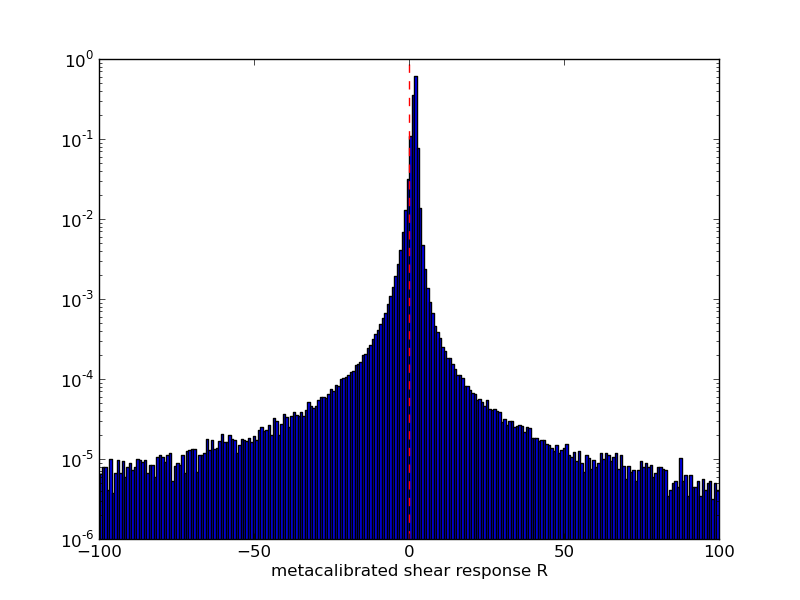
\includegraphics[width=0.45\textwidth]{./Plots/regauss-r-histogram.png}
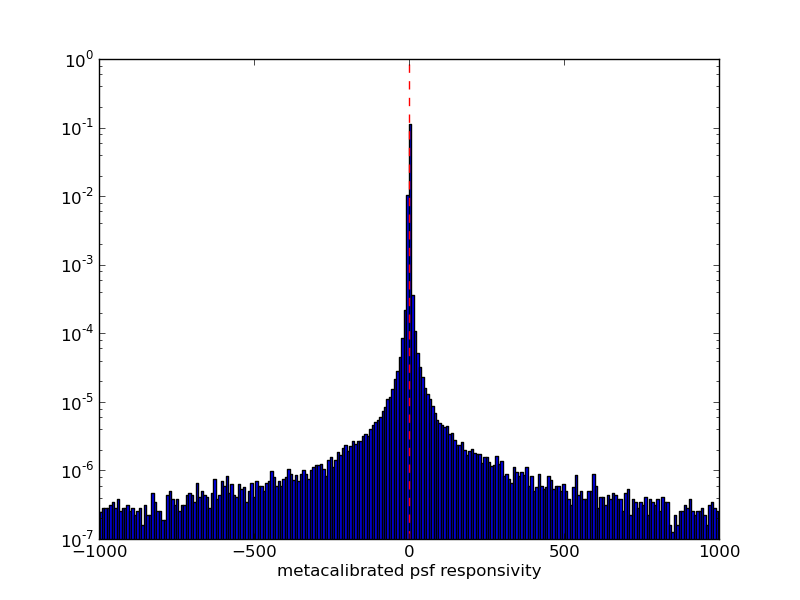
\includegraphics[width=0.45\textwidth]{./Plots/regauss-a-histogram.png}
\caption{{\bf Top:} Normalized distribution of meta-calibration shear
  responsivities from Regaussianization, on the
  Control-Ground-Constrant branch of the GREAT3 simulations.  {\bf
    Bottom:} Distribution of meta-calibration psf ellipticity
  responsivities from Regaussianization, on the
  Control-Ground-Constrant branch of the GREAT3 simulations. Vertical
  red dashed lines are drawn at zero for reference in both panels.}
\label{fig:calibhist}
\end{figure}


\begin{figure*}
\begin{center}
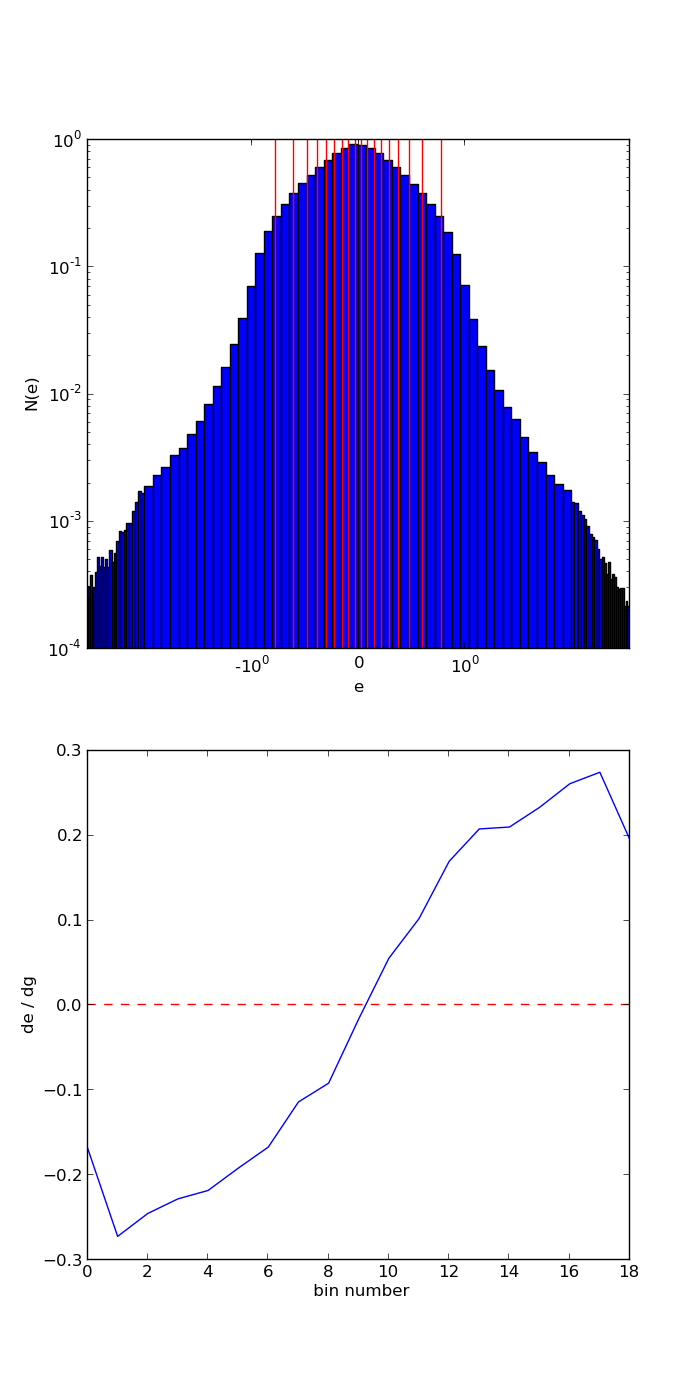
\includegraphics[width=0.3\textwidth]{./Plots/regauss-opt-shear_plots-prior_derivs.png}
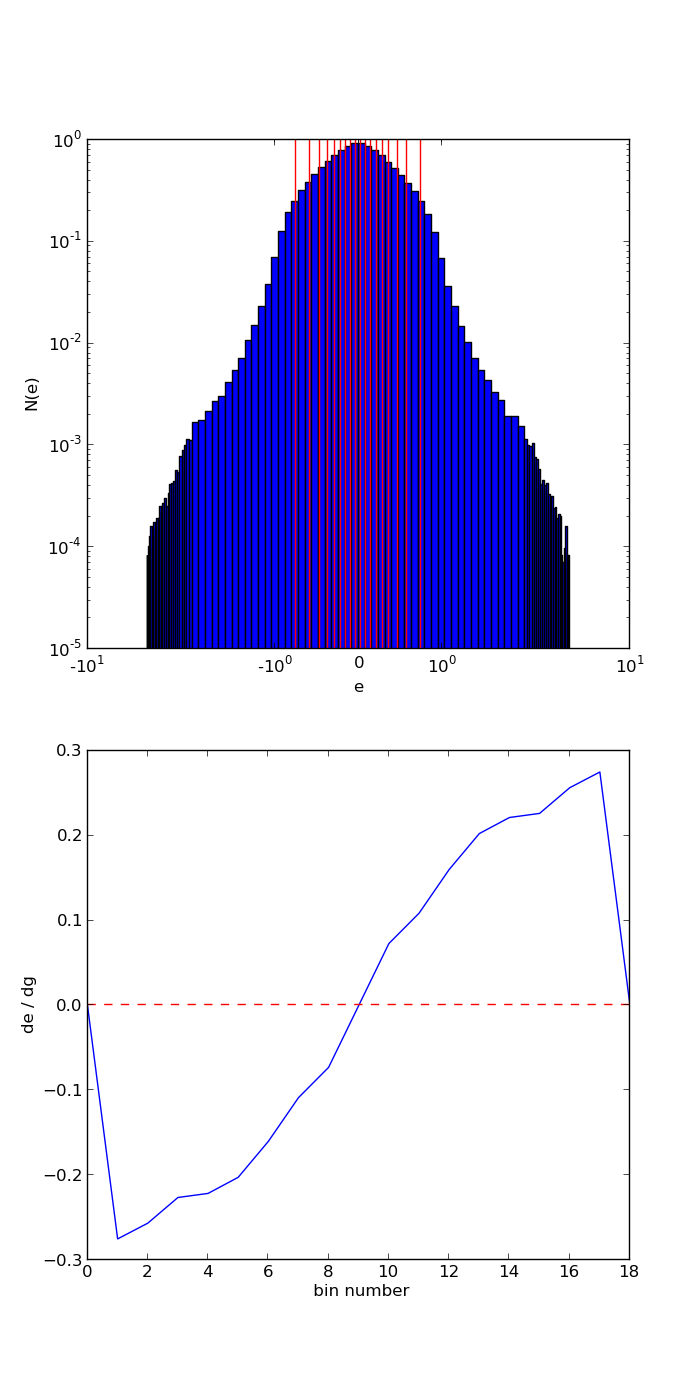
\includegraphics[width=0.3\textwidth]{./Plots/ksb-opt-shear_plots-prior_derivs.png}
\end{center}
\caption{I do not like these figures. Treat them as placeholders for now.\\
  Constructing the histogram estimator for the three shape measurement
  methods. {\bf Top} panels show measured shape distribution for the
  regauss ({\bf left}) and {\bf right} ksb algorithms. Vertical red
  lines show bin edges for a scheme with 20 bins, as used in the
  estimation. {\bf Bottom} panels show the derivative
  $\frac{d\,p(e)}{d{e}}$ for each of the histograms. Abscissa are
  truncated at $\pm 4$, but the estimator runs over bins including all
  objects. To stabilize the estimator, we set the values of the
  histogram derivatives in the outermost two bins to zero.}
\label{fig:estimator}
\end{figure*}

If we have a poor model for the unlensed histogram, $h_{\rm fid}$,
then the results will be biased. We can define a distance between each
field and the unlensed model using equation~\ref{eqn:multnomial},
taking the probabilities $q_i$ from the unlensed model and the
histogram amplitudes from the current field, after correcting for the
estimated shear. If the shear response measured for the unlensed prior
is correct, then the performance of the estimator will depend only on
the similarity of the model to the measurement field. The likelihood
can then be used as an objective criterion for the quality of the
inference.

\subsection{Relationship to previous implementations}

As shown in the GREAT3 results paper \citep{2015MNRAS.450.2963M}, an
early version of metacalibration was used in the GREAT3 challenge.
That implementation differs from the one presented here and released
publicly in association with this paper in two important ways: the
model for systematics was simpler than the one presented below (in
particular, it neglected additive systematics entirely) and the method
for inferring shears from an ensemble of objects was entirely
different.  These differences are of sufficient importance that the
GREAT3 results (especially the ones for additive systematics) are not
relevant to the implementation described here.


\section{Testing Framework}
\label{sec:testing}

\subsection{Estimation Algorithms}

Since the metacalibration method can in principle be used to calibrate
shears from any per-object shear algorithm, we chose three easily
available shear estimation methods, all of which are implemented in
GalSim.  Two of these methods are more traditional shear estimation
methods that have somewhat different assumptions but are both based on
object moments.  One method is not a standard shear estimation method
at all: we use linear combinations of the directly observed second
moments without correcting for the PSF at all.  In principle, the
information about how those respond to shear should be determined by
metacalibration to correctly infer the shear.  The difference in this
case is that instead of providing a small correction to the outputs of
a PSF correction method, we rely on metacalibration to do the entirety
of the PSF correction, which is a very stringent test.

\subsubsection{Regaussianization}

Re-Gaussianization \citep{2003MNRAS.343..459H} is a PSF correction
method based on the use of the moments of the image and of the PSF to
correct for the effects of the PSF on the galaxy shapes. It includes
corrections for the non-Gaussianity of the galaxy profile
\citep{2002AJ....123..583B,2003MNRAS.343..459H} and of the PSF (to
first order in the PSF non-Gaussianity). The performance of this
algorithm has been extensively studied in real data and simulations
\citep[e.g.,][]{2005MNRAS.361.1287M,2012MNRAS.420.1518M,2013MNRAS.432.1544M,2015MNRAS.450.2963M}.

The outputs of the re-Gaussianization algorithm are PSF-corrected
``distortions'', which for an object with purely elliptical isophotes
with minor-to-major axis ratio $q$ and position angle $\theta$ with
respect to the $x$ axis in pixel coordinates would be defined as
\begin{equation}
(e_1, e_2) = \frac{1-q^2}{1+q^2}\left(\cos{2\theta},\sin{2\theta}\right).
\end{equation}
As discussed in \cite{2002AJ....123..583B}, the response of a
distribution of galaxies with some intrinsic distribution of
distortions $p(e)$ to a shear is nonlinear in a way that depends on
the $p(e)$ itself.  Conceptually, we can think of an ensemble shear
estimator using re-Gaussianization outputs as
\begin{equation}
\hat{\gamma}_j = \frac{\langle e_j\rangle}{\mathrm{d}\langle e_j\rangle/\mathrm{d}\gamma_j}
\end{equation}
where the denominator gives the response of the ensemble average
distortion to a shear (often called the responsivity).  Estimators of
this shear responsivity use the observed galaxy $p(e)$ and its
moments, and for typical $p(e)$, the denominator is around
$1.7$--$1.8$.

\subsubsection{KSB}

The KSB method \citep{1995ApJ...449..460K} parametrises galaxies and
stars according to their weighted quadrupole moments.  The main
assumption of the KSB method is that the PSF can be described as a
small but highly anisotropic distortion convolved with a large
circularly symmetric function.  With that assumption, the shear can be
recovered to first-order from the observed ellipticity of each galaxy
via
\begin{equation} \label{eqn:weight}
\gamma=P_{\gamma}^{-1}\left(e^{\rm obs}-\frac{P^{\rm sm}}{P^{\rm sm*}}e^{*}\right),
\end{equation}
where asterisks indicate quantities that should be measured from the
PSF model at that galaxy position, $P^{\rm sm}$ is the smear
polarisability (see \citealt{2006MNRAS.368.1323H} for definitions) and
$P_\gamma$ is the correction to the shear polarisability that includes
the smearing with the isotropic component of the PSF. The
ellipticities are constructed from weighted quadrupole moments, and
the other quantities involve higher order moments. A circular Gaussian
weight of scale length $r_g$ is used, where $r_g$ is galaxy size.

The KSB method returns a per-object estimate of the shears
$(\hat{\gamma}_1, \hat{\gamma}_2)$. We can use metacalibration to
infer the shear while removing multiplicative and additive biases in
the method.

\subsubsection{Linear Moments}

As mentioned previously, the third method we use does not involve
PSF-corrected galaxy shapes.  Instead, we use linear combinations of
the second moments of galaxy images.  The motivation behind this
choice is as follows.  One way to estimate the distortion $(e_1,e_2)$
is via combinations of the second moments of the light profile,
\begin{equation}
\langle x_i\rangle = \frac{\int x_i w({\mathbf x}) I({\mathbf x}) \mathrm{d}^2{\mathbf x}}{\int w({\mathbf x}) I({\mathbf x}) \mathrm{d}^2{\mathbf x}}
\end{equation}
for $i=1, 2$,
\begin{equation}
M_{ij} = \frac{\int (x_i-\langle x_i\rangle)(x_j-\langle x_j\rangle) w({\mathbf x}) I({\mathbf x}) \mathrm{d}^2{\mathbf x}}{\int w({\mathbf x}) I({\mathbf x}) \mathrm{d}^2{\mathbf x}}
\end{equation}
for $i,j=1,2$, and finally 
\begin{equation}\label{eq:moments-div}
e_1 = \frac{M_{11}-M_{22}}{M_{11}+M_{22}}, \qquad e_2 \frac{2M_{12}}{M_{11}+M_{22}}.
\end{equation}

One source of noise in traditional moments based methods is the
division of two noisy quantities in Eq.~\ref{eq:moments-div},
typically followed by further division by other noisy quantities to
remove the dilution of the galaxy shape by the PSF.  Thus, as a final
example of a statistic that we will attempt to use as a calibrated
shear estimator with metacalibration, we define the following linear
combinations of moments:
\begin{equation}
\hat{M}_i = (M_{11}-M_{22}, 2M_{12}).
\end{equation}

Clearly these moments are sensitive to a number of nuisance
quantities, like the galaxy flux and size.  They also do not include
any PSF correction whatsoever.  In principle, metacalibration should
be able to nonetheless determine the response of this statistic to
shear, $\mathrm{d}\hat{M}_i/\mathrm{d}\gamma$, and produce a reliable
shear estimate, provided that the model for the predominant sources of
systematics follows that in Eq.~\ref{eqn:edist_model}.  This is a
quite stringent test of the metacalibration method.

\subsection{Simulated Images}

We use the GREAT3 simulation framework as the source of simulated
images that we use for testing purposes.  For more detail about that
simulation framework, see the GREAT3 handbook
\citep{2014ApJS..212....5M} and results paper
\citep{2015MNRAS.450.2963M}, or the publicly available
software\footnote{\url{https://github.com/barnabytprowe/great3-public}}.

In brief, we use simulated ``branches'' containing 200 ``subfields''.
Each subfield contains $10^4$ galaxies placed on a $100\times 100$
grid; the galaxies in a given subfield all have the same (unknown)
shear and the same known PSF.  The galaxy population within a subfield
follows a distribution of signal-to-noise ratio, size, ellipticity,
and morphology based on that in the {\it Hubble Space Telescope} ({\it
  HST}) COSMOS survey
\citep{2007ApJS..172..196K,2007ApJS..172....1S,2007ApJS..172...38S},
roughly approximating a galaxy sample with a depth of $I<25$.  To
ensure that most methods will be able to measure all galaxies, an
effective signal-to-noise cut of $\gtrsim 12$ and a minimal resolution
cut was imposed (resulting in different sets of galaxies in subfields
that have different-sized PSFs).  90$^\circ$ rotated pairs of galaxies
were included, to cancel out shape noise \citep{2007MNRAS.376...13M}.
The PSF in the simulations comes from the combination of an optics
model from a ground-based telescope, along with a Kolmogorov PSF with
a typical ellipticity variance.  Thus, the galaxy and PSF properties
are non-trivially complicated.  The noise is stationary Gaussian
noise.  The ultimate goal is to estimate the average shear in each
subfield in an unbiased way, without any multiplicative bias or
correlations with the per-subfield PSF ellipticity.

One important distinction between GREAT3 and the real Universe that we
will have to consider is the mean shear.  In a real patch of sky
comparable to the size of a large survey, the expected mean shear is
zero.  In GREAT3, while lensing shears $g_1$ and $g_2$ are drawn from
a distribution with zero mean, the fact that there are only 200
subfields means that effectively only 200 draws from that distribution
were made, and that is not enough to have an effective mean shear of
zero.  Thus, for all of the results below, we will take the averages
of the true shears per component as a known quantity instead of doing
a fully blind analysis, since the deviation of those quantities from
zero is just due to the artificial nature of the simulation design.

We consider two sets of galaxy populations.  One comes directly from
{\it HST} images, and includes a process to remove the HST PSF before
shearing (both operations being carried out in Fourier space) and
convolving with the final target PSF \citep{2012MNRAS.420.1518M}.  The
other galaxy population consists of simple parametric representations
of those {\it HST} images.  These populations have the same effective
distributions of size, ellipticity, and so on, but one includes
realistic galaxy morphology while the other only includes such realism
as can be captured by the sum of two S\'{e}rsic profiles.  In the
language of GREAT3, we use simulations corresponding to
control-ground-constant (describing the parametric galaxy sample,
ground-based simulated data, with a constant per-subfield shear) and
real$\_$galaxy-ground-constant (the realistic galaxy sample), denoted
CGC and RGC.


\subsubsection{Control Ground Constant without Aberrations}

Before analyzing the GREAT3 results, we analyze a newly-generated set
of simulations that is closely analogous to the GREAT3 CGC branch
(parametric galaxy profiles), but with one modification to avoid a
problem raised in the results paper \citep{2015MNRAS.450.2963M}.
There, it was noted that the CGC branch has a number of outlier fields
related to unusually large optical PSF aberrations, specifically
defocus and trefoil.  Thus, our first simulated dataset is designed
exactly like CGC but with all aberrations in the optical PSF set to
zero, to ensure reasonable consistency of data quality.  Note that the
atmospheric PSF is still drawn from a distribution of seeing values
for each subfield.

\subsubsection{Real Ground Constant without Aberrations}

The next branch we analyze is similar to the previous one, but with
realistic galaxies.  Thus, we refer to this branch as ``RGC without
aberrations''. This lets us separate the effects of realistic galaxy
morphology from the problems inherent in correcting a complex PSF. For
this branch, it is not necessary to use a likelihood cut to remove
fields with aberrant psf behavior in defining the null ellipticity
distribution, and so we include all branches in our analysis.

As seen in Table \ref{table:results}, the percent-level shear
calibration biases for regauss on this branch are reduced by MetaCal
to a level consistent with zero. No trend with PSF ellipticity is
detected before or after detrending. Realistic galaxy morphologies do
not appear to have a significant impact on our correction procedure.


\subsubsection{Control Ground Constant}

After testing metacalibration on the simulations without aberrations,
we now turn to the actual GREAT3 simulated data in the CGC branch,
including parametric galaxies.

For this branch, we have tested the performance of MetaCal on all
three shape estimation algorithms described in Section
\ref{sec:testing}. Figures \ref{fig:cgc_uncorrected} and \ref{fig:cgc_corrected}
show the results of shear estimation with
and without metacalibration for each algorithm. In all three cases,
our technique has substantially reduced shear calibration biases below
their uncorrected levels. The linear moments, in particular carry
almost no useful shear information in the absence of metacalibration;
after correction, their performance is superior to that of uncorrected
KSB.

Also notable in these figures is the fact that residual psf trends
after metacalibration tend to be driven by fields with very large psf
ellipticity. These could be (and often would be) excluded in a real
analysis. 


\begin{figure*}[t]
\begin{center}
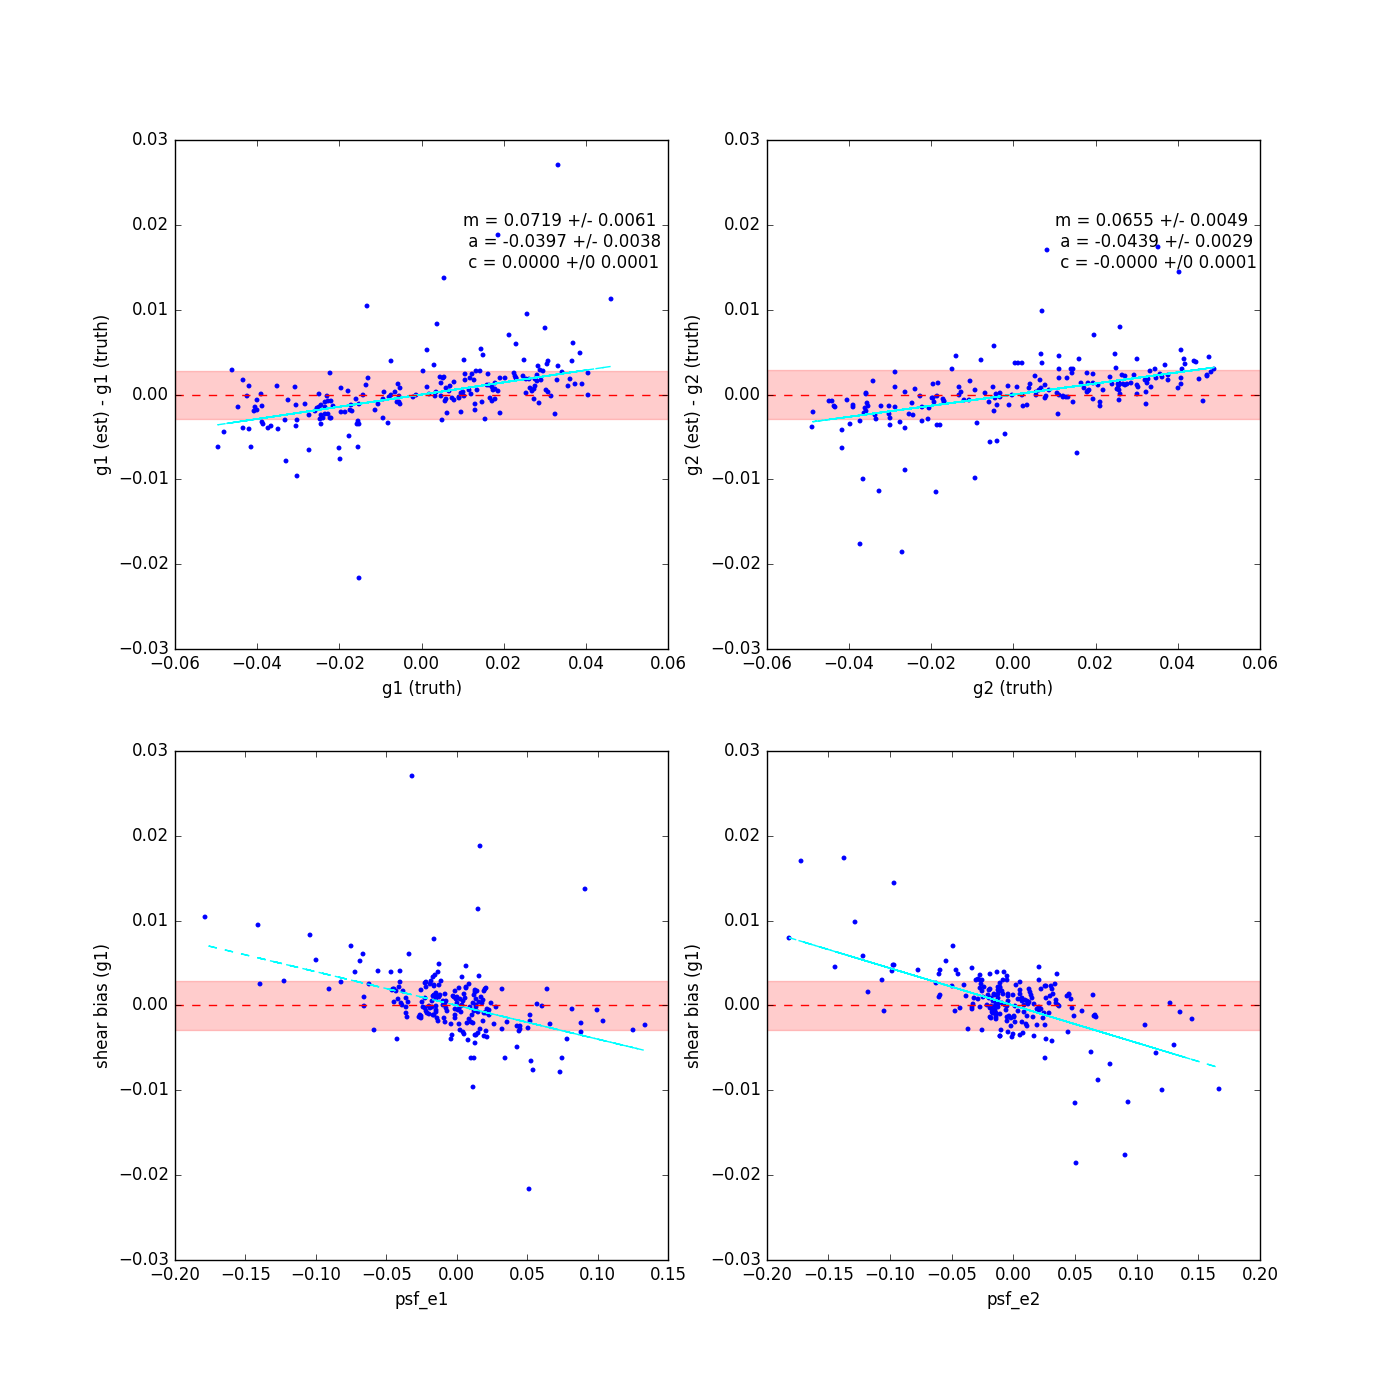
\includegraphics[width=0.32\linewidth]{./Plots/regauss-no_corrections.png}
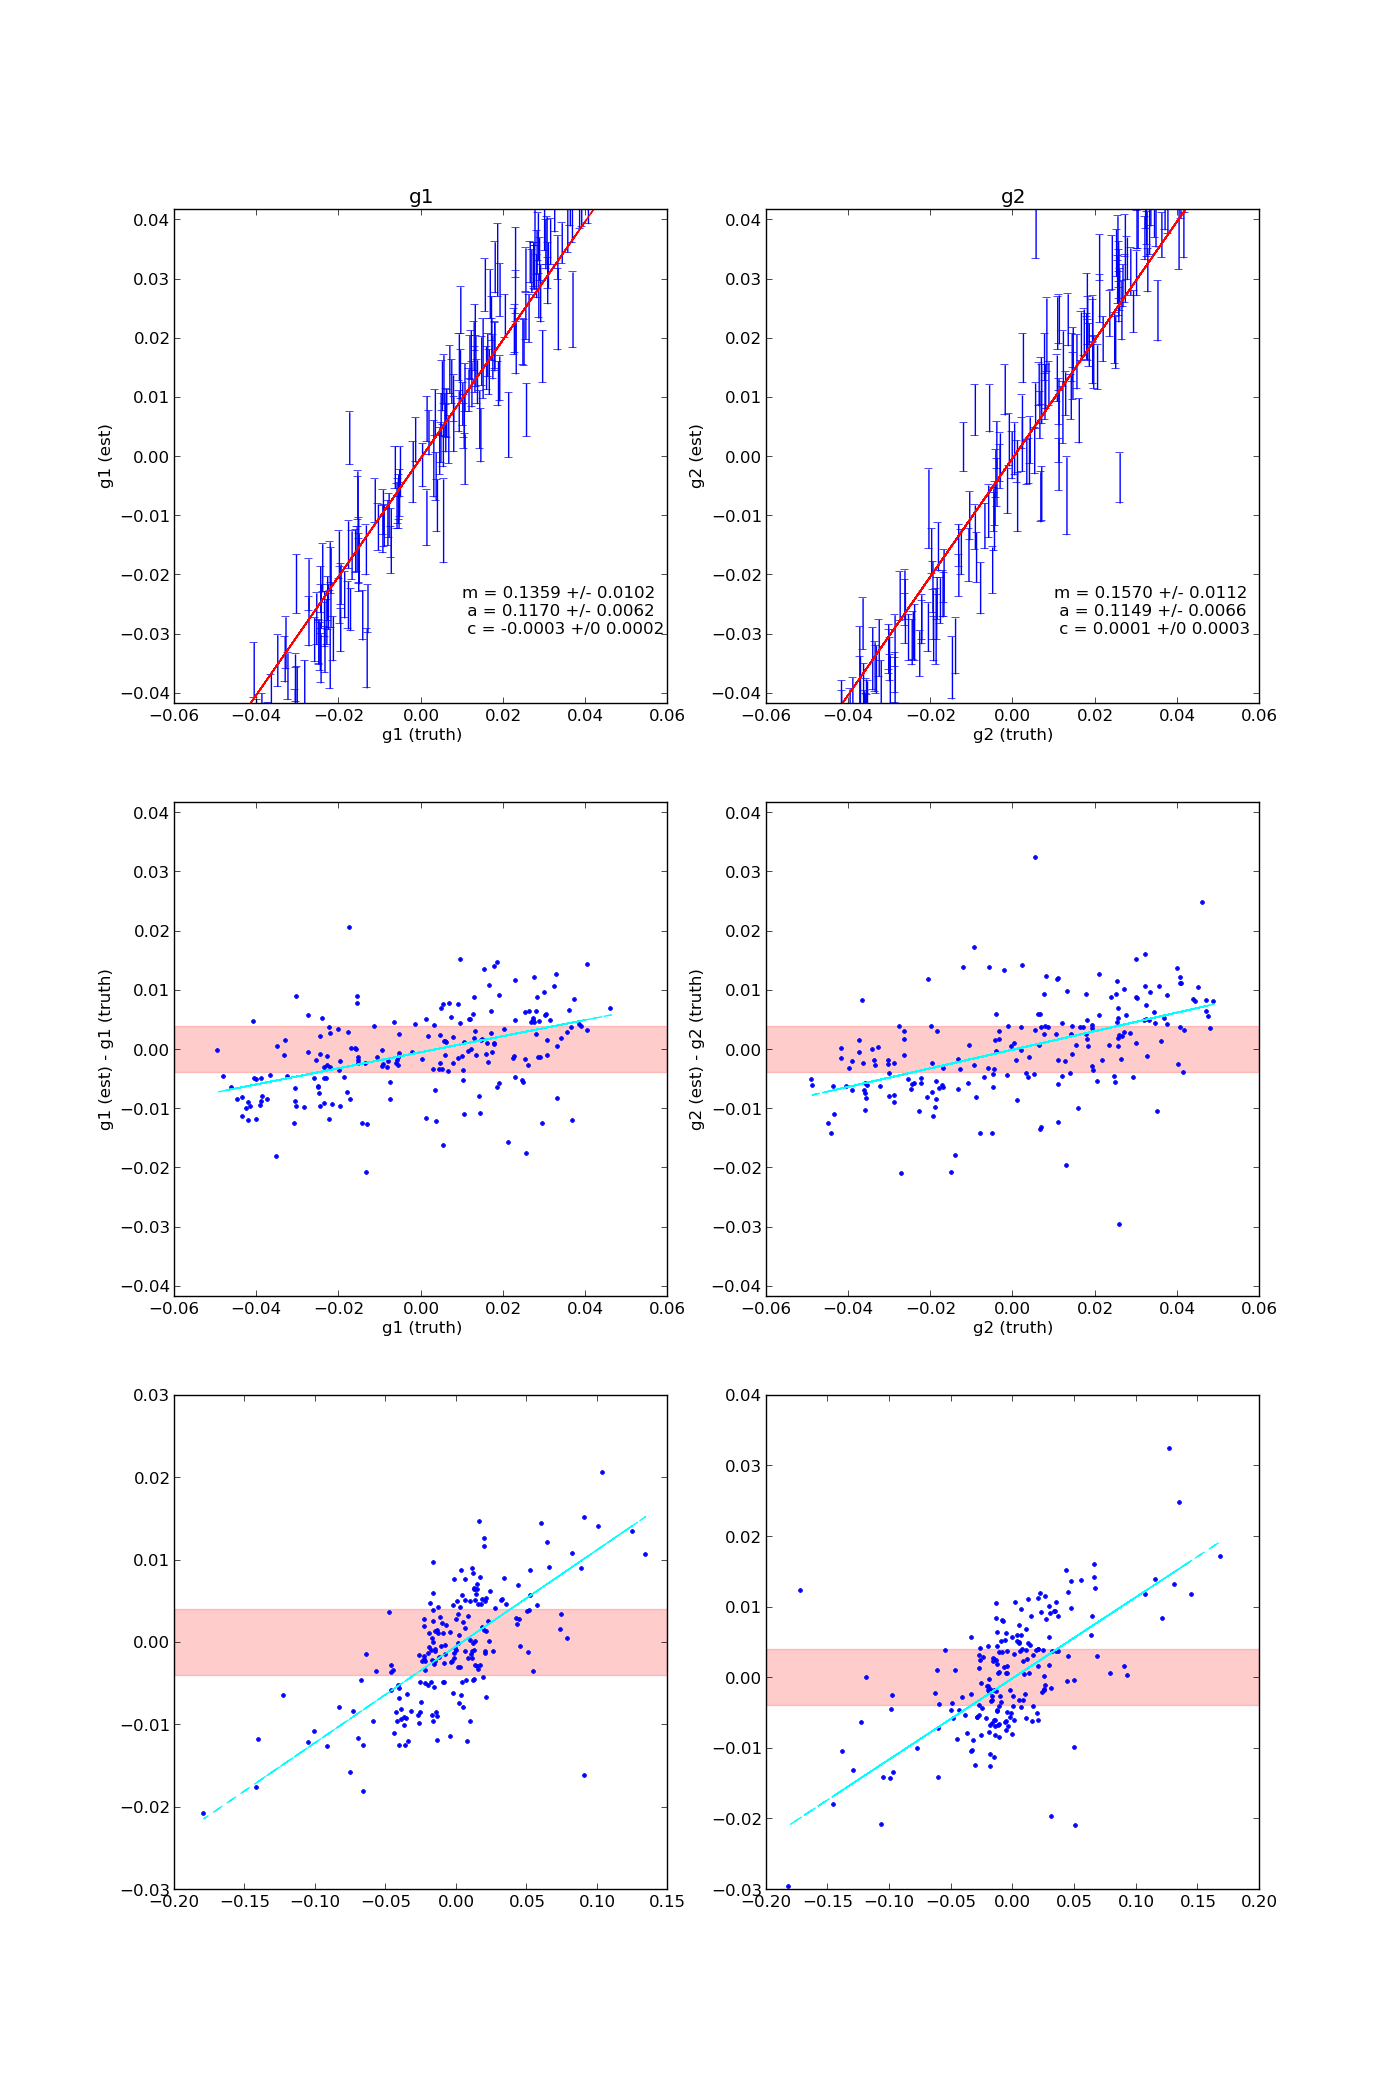
\includegraphics[width=0.32\linewidth]{./Plots/ksb-no_corrections.png}
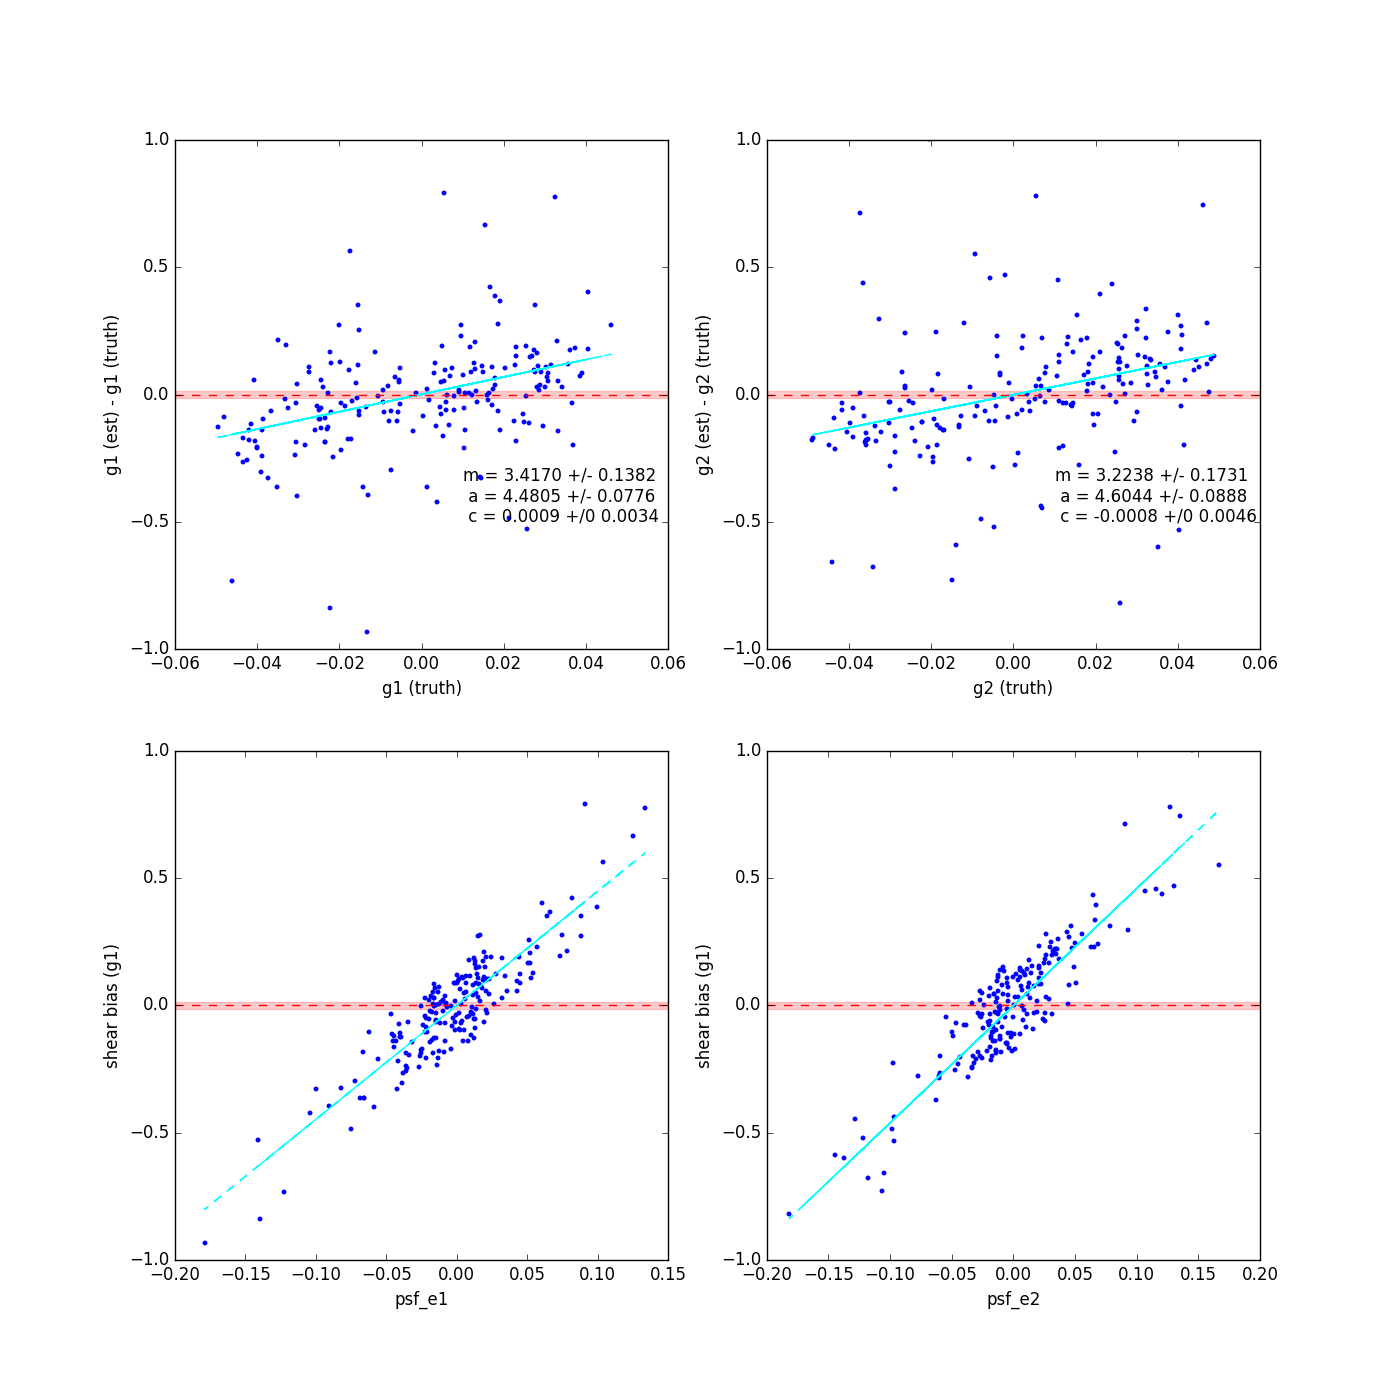
\includegraphics[width=0.32\linewidth]{./Plots/moments-no_corrections.png}
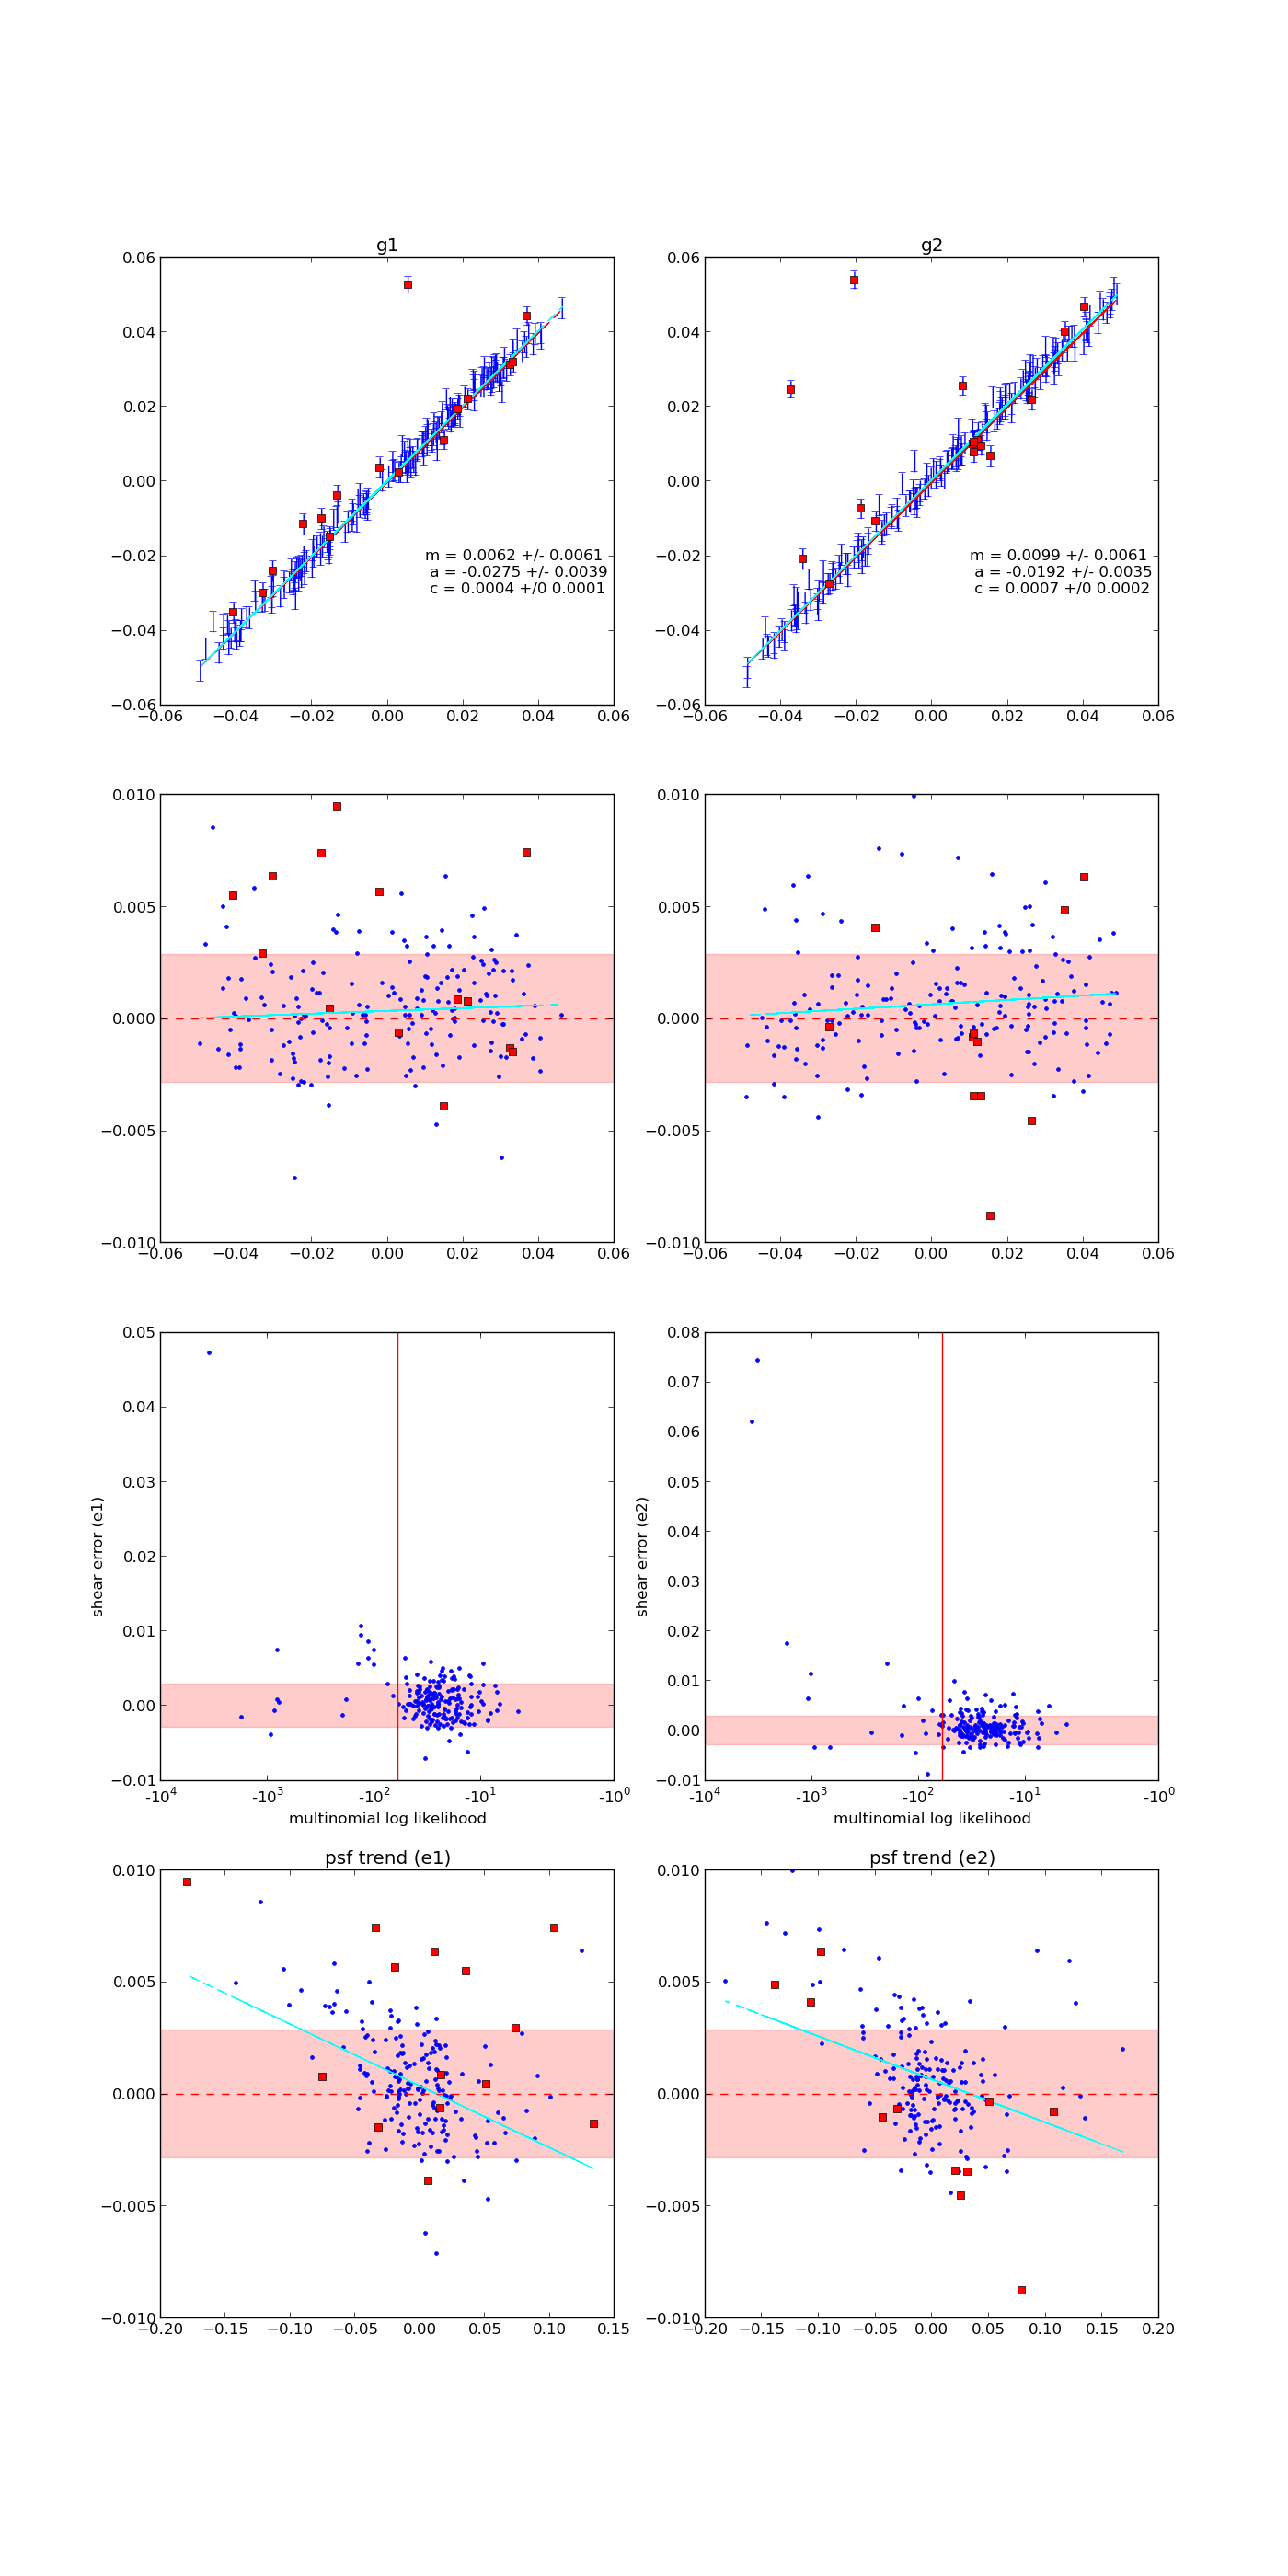
\includegraphics[width=0.32\linewidth]{./Plots/regauss-opt-shear_plots.png}
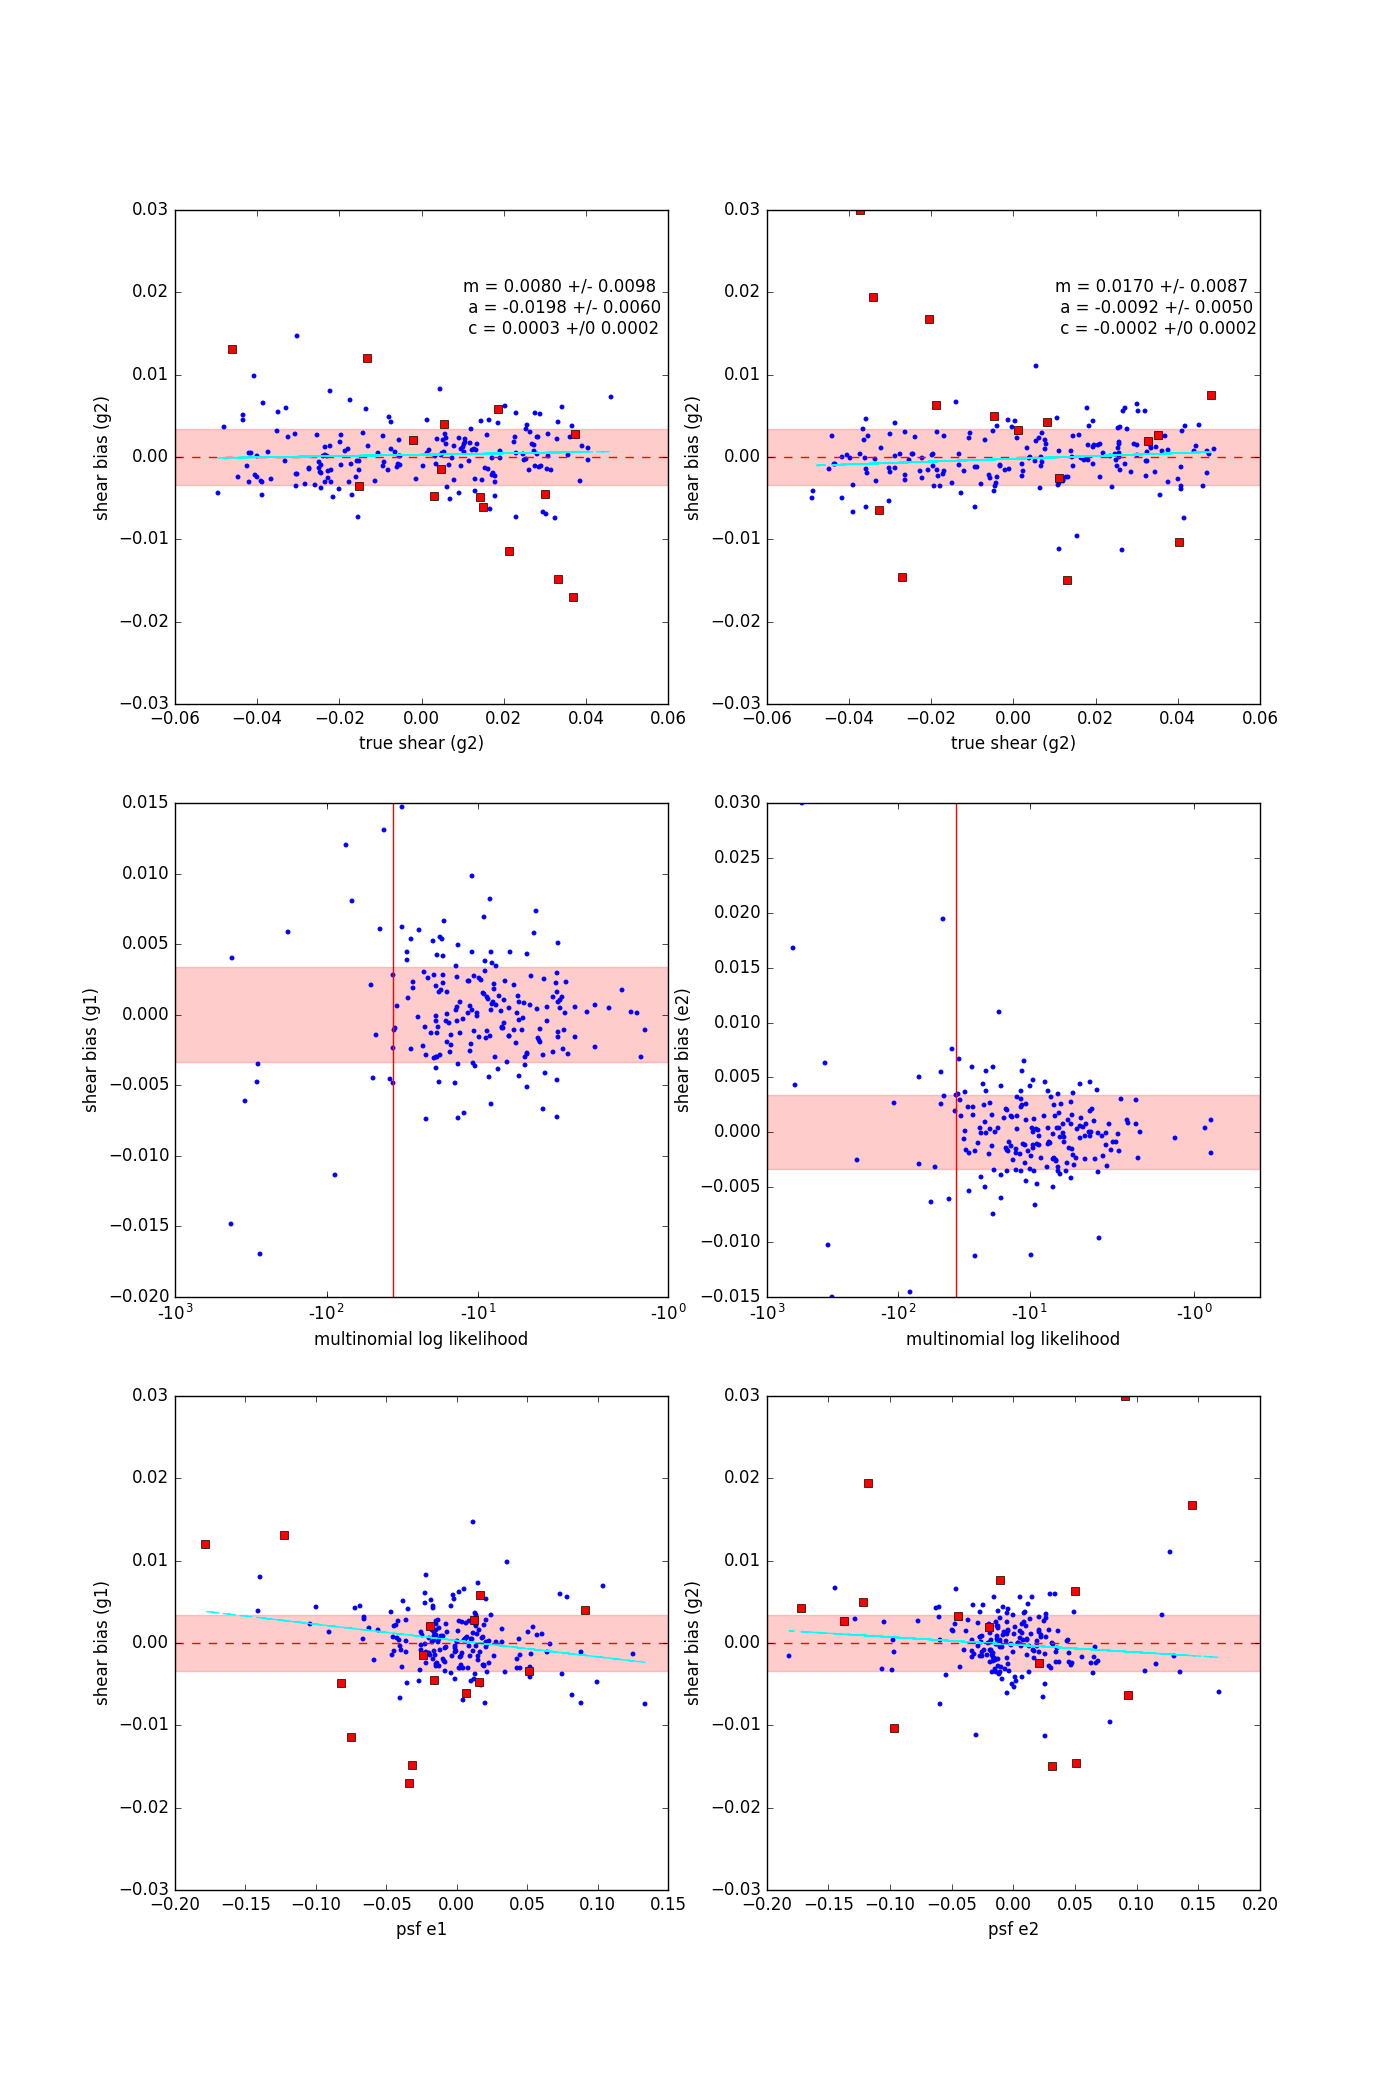
\includegraphics[width=0.32\linewidth]{./Plots/ksb-opt-shear_plots.png}
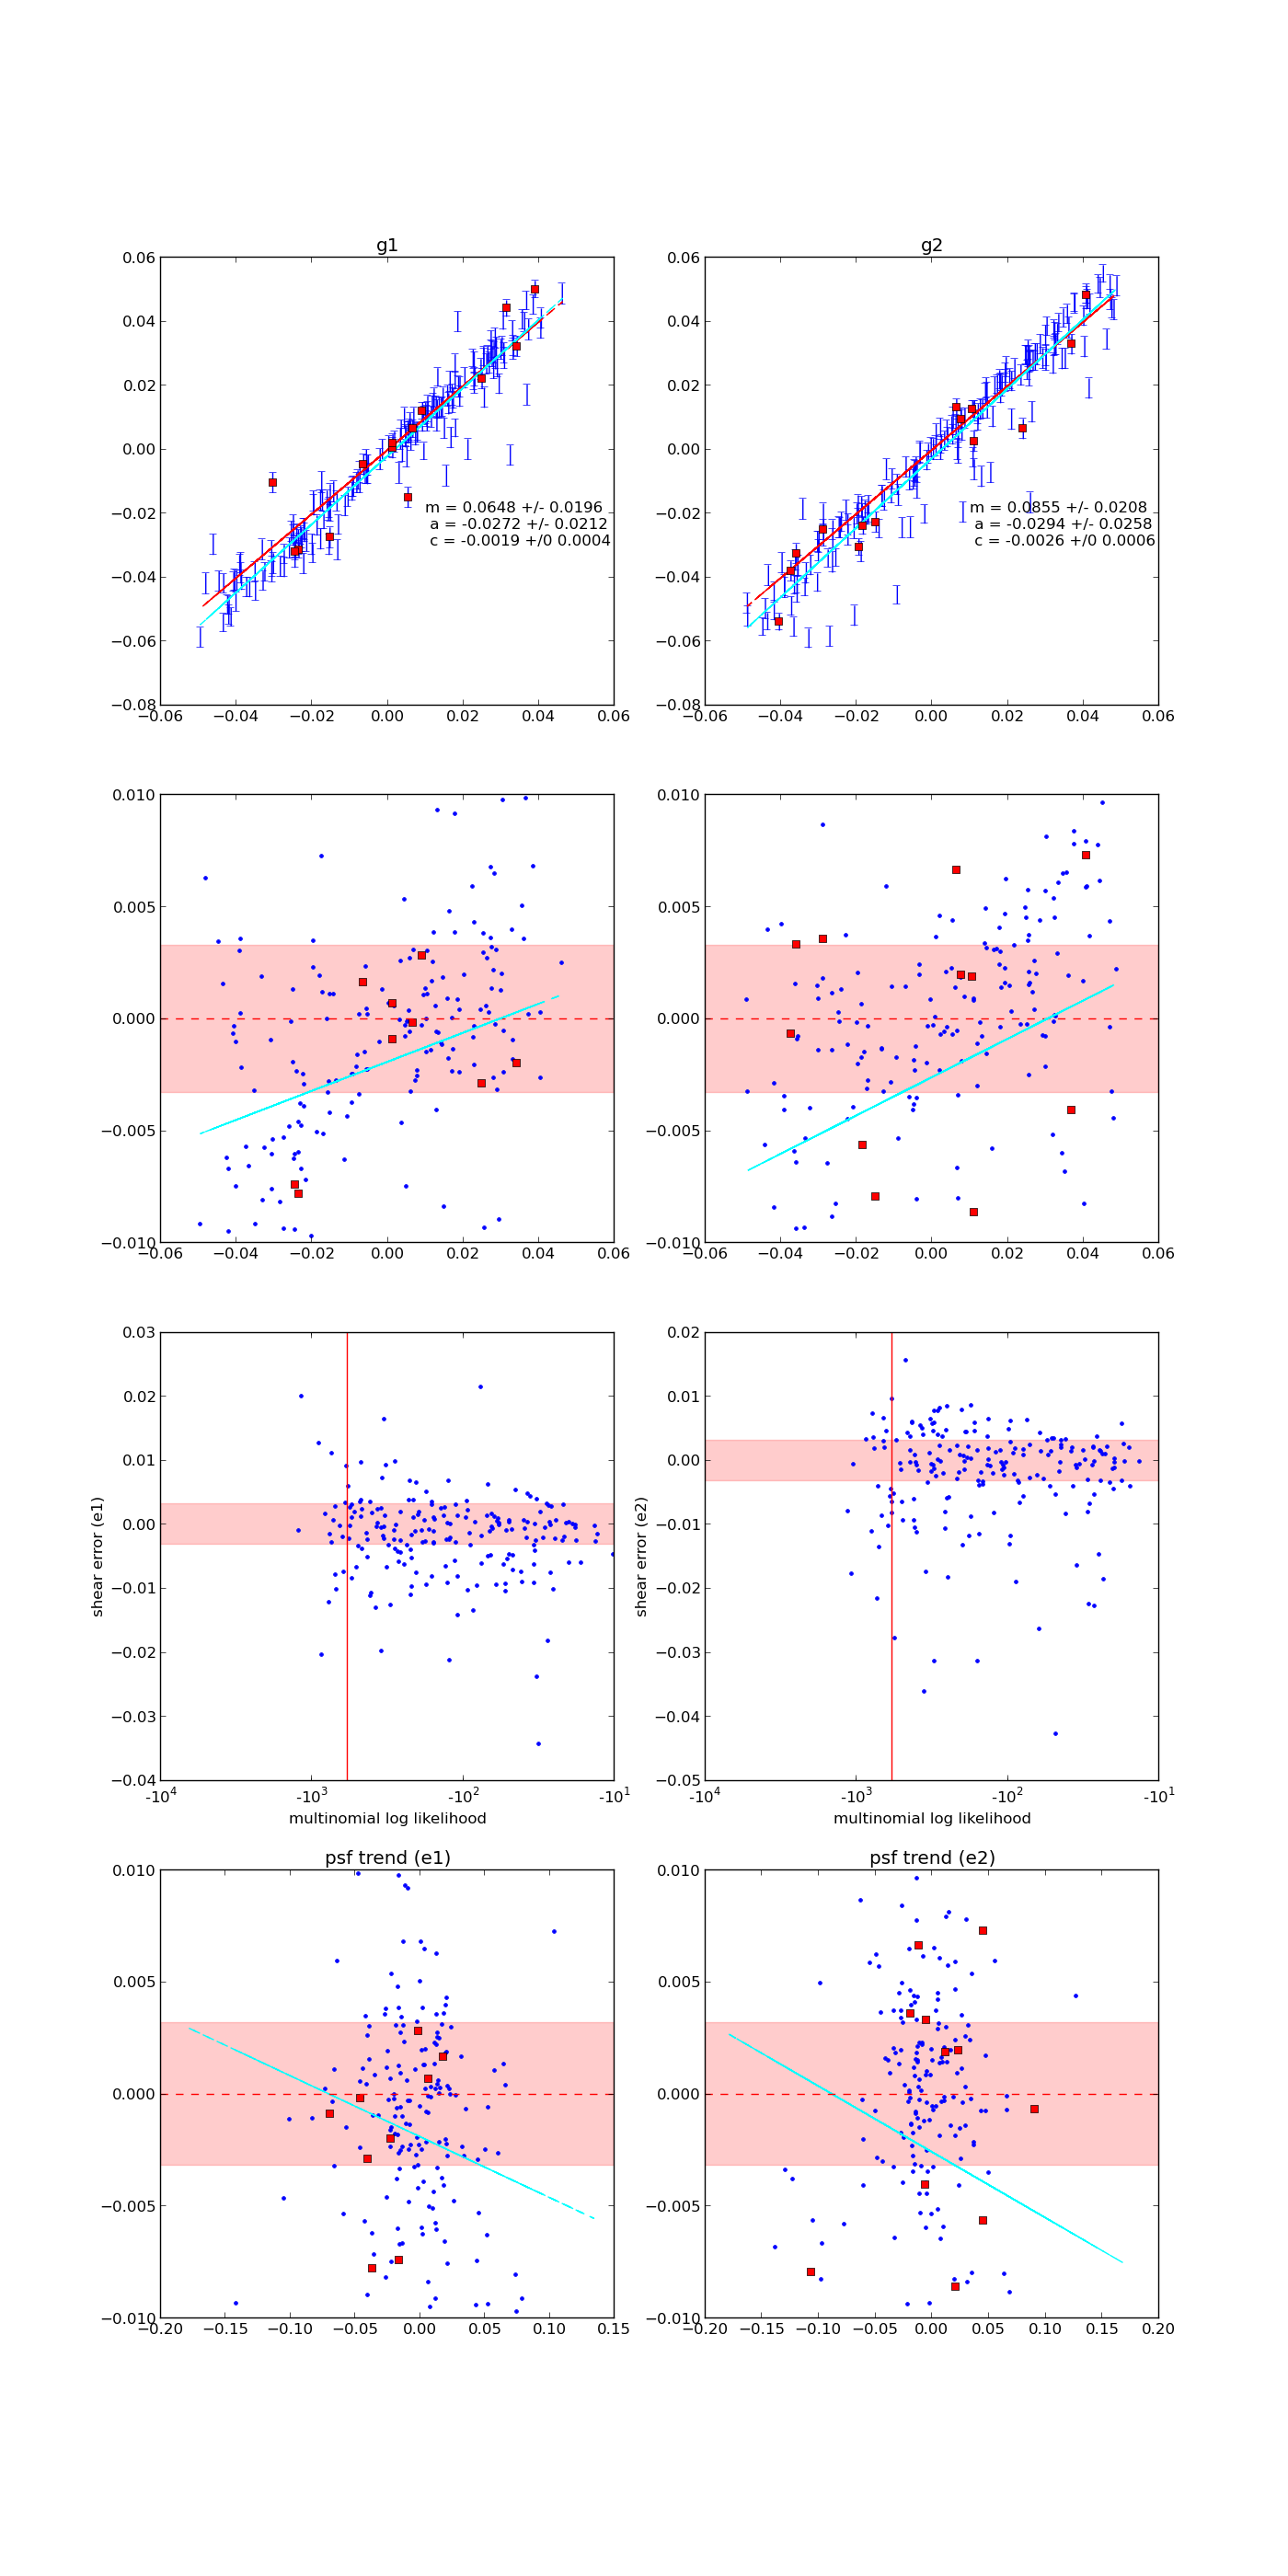
\includegraphics[width=0.32\linewidth]{./Plots/moments-opt-shear_plots.png}
\end{center}
\caption{{\bf Top:} Results {\it without} metacalibration for the regauss ({\bf left}), KSB ({\bf
    center}), and Linear Moments ({\bf right}) algorithms on the CGC.
  branch.  {\bf Bottom:} Results {\it with} metacalibration for the regauss ({\bf left}), KSB ({\bf
    center}) and Linear Moments algorithms ({\bf right}) on CGC.}
\label{fig:cgc_corrected}
\end{figure*}




\subsubsection{Real Ground Constant}

Next, we analyze the actual GREAT3 simulations in the RGC branch, with
realistic galaxy morphology. Here the metacalibrated regaussianization
results continue to be consistent with no shear calibration bias. The
KSB results retain a noticeable calibration error, but it has again
been reduced by a factor of $\sim3-4$ below its uncorrected value. 



\subsubsection{Real Ground Constant with constant aberrations}

One issue of concern is how to understand outlier fields.  In GREAT3,
there was a concern that some outliers were due to failure of our
model for interpreting the per-object shapes in fields that had large
aberrations.

As a way to understand this, we generated a version of RGC that had
quite large aberrations that were identical in each field:
specifically defocus of $0.5$ waves and one component of trefoil of
$0.1$ wave.

This removes the difficulties in building a null ellipticity
distribution, isolating the impact of a complex PSF. Here the results
remain very positive: metacalibration removes the $\sim0.06$ shear
calibration bias, and successfully eliminates the small residual psf
ellipticity trend in the uncorrected regauss results.


\section{Results}
Metacalibration is a perturbative technique that appears to work best
on shear estimation algorithms with small calibration biases. Those
cases we have examined where the initial biases are large or not
linear are not completely corrected by our linear detrending scheme,
though in every case we have studied the algorithm appears to
substantially improve biases resulting from faulty PSF correction and
shear miscalibration. Even the nearly information-free linear moments
algorithm appears to be calibrated by our procedure to a level
superior to a KSB, a widely used traditional shear estimation algorithm.


\begin{figure*}
\makebox[\textwidth][c]{
\begin{tabular}{l  c |cc | cc |cc }
\hline
branch & algorithm  &  $m_1$ & $m_2$  & $a_1$ & $a_2$ &  $c_1$ & $c_2$ \\
\hline
\hline
CGC & regauss (MC)  & $0.0036 \pm 0.0072$ & $0.0023\pm0.0064$ & $-0.0206\pm0.0046$ & $-0.0194\pm0.0036$ &  $0.0000\pm0.0002$ & $0.0001\pm0.0002$ \\
CGC & regauss  &  $0.0719\pm0.0061$ & $0.0655\pm0.0049$  & $-0.0397\pm0.0038$ & $-0.0439\pm0.0029$ &  $0.0000\pm0.0001$ & $0.0000\pm0.0001$ \\
CGC & ksb (MC)  &  $0.0080\pm0.0098$ & $-0.0170\pm0.0087$  & $-0.0198\pm0.0060$ & $-0.0092\pm0.0050$ &  $0.0003\pm0.0002$ & $-0.0002\pm0.0002$ \\
CGC & ksb  &  $0.1322\pm0.0088$ & $0.1455\pm0.0104$  & $0.1148\pm0.0054$ & $0.1096\pm0.0061$ &  $-0.0004\pm0.0002$ & $0.0000\pm0.0003$ \\
CGC & moments (MC) & $0.0371\pm0.0173$ & $0.0459\pm0.0184$ & $-0.0880\pm0.0099$ & $-0.0877\pm0.0095$ & $0.0001\pm0.0004$ & $-0.0002\pm0.0005$\\
CGC & moments & $3.4170\pm0.1382$ & $3.2238\pm0.1731$ & $4.4805\pm0.0776$ & $4.6044\pm0.0888$ & $0.0009\pm0.0034$ & $-0.0008\pm0.0046$ \\
RGC & regauss (MC) &  $-0.0053\pm0.0078$ & $0.0061\pm0.0066$  & $0.0036\pm0.0040$ & $-0.0031\pm0.0037$ &  $0.0001\pm0.0002$ & $0.0001\pm0.0002$ \\
RGC & regauss &  $0.0304\pm0.0052$ & $0.0249\pm0.0050$  & $-0.0295\pm0.0028$ & $-0.0186\pm0.0028$ &  $0.0000\pm0.0001$ & $0.0002\pm0.0001$ \\
CGC-Noaber & regauss (MC)  &  $-0.0074\pm0.0069$ & $0.0061\pm0.0064$  & $-0.0339\pm0.0127$ & $-0.0237\pm0.0112$ &  $0.0001\pm0.0002$ & $0.0001\pm0.0002$ \\
CGC-Noaber & regauss  &  $0.0407\pm0.0029$ & $-0.0439\pm0.0029$  & $-0.0274\pm0.0052$ & $-0.0265\pm0.0050$ &  $0.0001\pm0.0001$ & $0.0001\pm0.0001$ \\
RGC-Noaber & regauss (MC)&  $0.0075\pm0.0050$ & $0.0140\pm0.0048$  & $-0.0188\pm0.0096$ & $-0.0108\pm0.0091$ &  $0.0000\pm0.0001$ & $0.0000\pm0.0001$ \\
RGC-Noaber & regauss &  $0.0164\pm0.0030$ & $0.0174\pm0.0034$  & $0.0022\pm0.0058$ & $0.0025\pm0.0064$ &  $0.0002\pm0.0001$ & $0.0000\pm0.0001$ \\
RGC-FixedAber & regauss (MC) &  $-0.0047\pm0.0089$ & $0.0060\pm0.0072$  & $-0.0154\pm0.0221$ & $-0.0160\pm0.0175$ &  $0.0001\pm0.0002$ & $-0.0002\pm0.0002$ \\
RGC-FixedAber  & regauss  &  $0.0616\pm0.0066$ & $0.0637\pm0.0052$  & $-0.03\pm0.0121$ & $-0.0323\pm0.0135$ &  $0.0003\pm0.0002$ & $0.0000\pm0.0001$ \\
\hline
\end{tabular}
}
\caption{Shear and psf calibration bias parameters from each of the
  branches considered. Rows with MetaCalibrated parameters are shown
  above their un-calibrated counterparts. Note that in every case,
  MetaCalibrating removes multiplicative biases within the precision
  allowed by the simulation volume, and reduces the amplitude of psf
  calibration biases.}
\label{table:results}
\end{figure*}

\section{Applicability to Real Data}
Several implementation issues need to be solved before this method can
be deployed on real survey data. We have made no attempt to deal with
the effects of masked pixels or blending, and while it seems clear
that our proposed algorithm has the potential to deal with selection
biases, we have not demonstrated that capability here.  The simulated
galaxies used in the GREAT3 simulations are arranged to cancel shape
noise, which would tend to eliminate additive measurement
biases. While we do not see any reason why metacalibration
measurements would be susceptible to additive biases, these
simulations do not provide strong evidence to that effect. Finally,
the average signal-to-noise of the GREAT3 galaxies is higher than that
of those currently used for shear estimation in the Dark Energy
Survey, so it is possible that noise rectification biases may become
significant when this is applied to realistic catalogs.

In a follow-up paper (Sheldon et al. 2016) we will demonstrate
algorithmic improvements that allow this technique to be used on Dark
Energy Survey data with state-of-the-art shear estimation algorithms.

\section{Conclusions}
We have described a new technique for introducing synthetic lensing
signal into real data, and shown that our algorithm can be used to
remove shear calibration biases while making almost no assumptions
about the properties of the galaxies in the data. This works because
the images depend linearly on the shear in the limit of interest for
weak lensing, while the shear catalogs that ultimately result from
subsequent measurement and processing have a much less straightforward
functional dependence on the signal.

We also argue that simple extensions of this approach are likely to be
able to deal with important sources of calibration bias that are not
easily testable in the GREAT3 simulations. Shear-dependent selection
biases are difficult to constrain with existing techniques, as they
require a realistic model for the ensemble properties of the galaxies
at the boundary of the sample selection. If metacalibration is applied
before the detection and selection steps, however, the estimated shear
calibration will include selection biases. Noise biases -- in
particular the effects of the correlated noise produced by our image
manipulations -- are also likely to matter for galaxies at
signal-to-noise ratios lower than those simulated in GREAT3.

In the forthcoming Sheldon et al. 2016, we will test metacalibration
on a larger and more realistic set of image simulations, and examine
whether this new technique can address the remaining sources of
calibration bias untested in GREAT3.




\section*{Acknowledgments}


\bibliographystyle{apj}
\bibliography{bibliography}


\end{document}
